\section{相位噪声和I/Q不平衡模型}
    
    \frame{\sectionpage}
    
    \begin{frame}{\textbf{I/Q不平衡模型}}
   		\begin{block}{理想情况下:给定基带I/Q信号$x(t) = x_I(t)+jx_Q(t)$}
   		\begin{itemize}
   			\item 上变频得到$x_p(t) = x_I(t)\cos(2\pi f_ct) - x_Q(t)\sin(2\pi f_ct)$
   			\item 下变频还原到$x(t) = x_I(t)+jx_Q(t)$.
   		\end{itemize}
   		\end{block}
   	
   		同向和正交两路中, 其相对幅度可能发生不该有的变化. 这会带来我们的 I/Q 不平衡现象.
   	
	\end{frame}
    
    \begin{frame}{\textbf{I/Q不平衡模型}}
    上变频和下变频的过程中,都会带来I/Q不平衡.
    \begin{block}{带有I/Q不平衡时:对基带I/Q信号$x(t) = x_I(t)+jx_Q(t)$}
    	\begin{itemize}
    		\item 上变频得到$\tilde{x}_p(t) = \alpha_{I,tx}x_I(t)\cos(2\pi f_ct) - \alpha_{Q,tx}x_Q(t)\sin(2\pi f_ct)$
    		\item 下变频得到$\tilde{x}(t) = \frac{\alpha_{I,rx}+\alpha_{Q,rx}}{2}x(t) + \frac{\alpha_{I,rx}-\alpha_{Q,rx}}{2}x^*(t)$.
    	\end{itemize}
    \end{block}
    
   	该信号的频谱中产生了一个镜像的频率干扰
   	\begin{equation}
   		\tilde{X}(f) = \frac{\alpha_{I,rx}+\alpha_{Q,rx}}{2}X(f) +  \frac{\alpha_{I,rx}-\alpha_{Q,rx}}{2} X^*(-f)
   	\end{equation}
    
\end{frame}
    
    \begin{frame}{\textbf{I/Q不平衡模型}}
    	\begin{columns}[T] % align columns
    		\begin{column}<0->{.40\textwidth}
    			\begin{figure}[thpb]
    				\centering
    				\resizebox{1\linewidth}{!}{
    					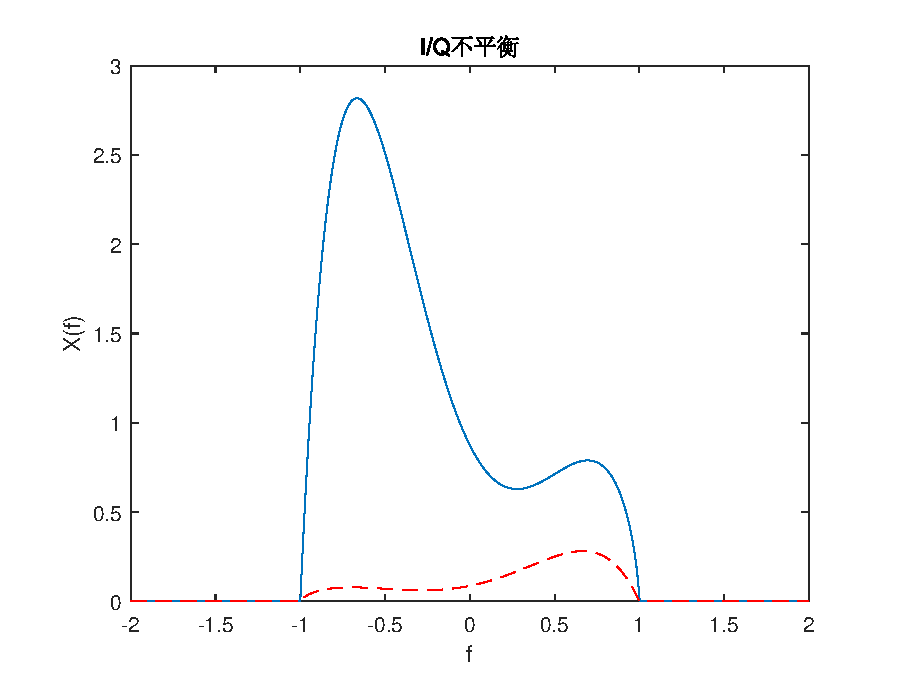
\includegraphics{images/IQ.eps}
    				}
    				%\includegraphics[scale=1.0]{figurefile}
    				$\quad$\caption{I/Q不平衡带来的镜频干扰}
    				\label{fig:campus}
    			\end{figure}
    		\end{column}%
    		\hfill%
    		\begin{column}<0->{.5\textwidth}
    			\begin{itemize}
    				\item 实际的 OFDM系统的上、下变频模块中,这种I/Q不平衡的效应则将会影响镜像位置处的子载波信道中的信号
    				\item I/Q不平衡效应还会使我们错误地估计需要去耦合的那部分发送信号,从而导致自干扰消除后仍然有一部分自干扰残余的出现. 
    			\end{itemize}
    		\end{column}%
    	\end{columns}
	\end{frame}

	\begin{frame}{\textbf{相位噪声模型}}
		\begin{block}{自激(FRO)振荡器模型的相位噪声假定为一个布朗运动}
			\begin{itemize}
				\item 相位噪声的复数振荡器可以描述为$\alpha_{OSC}(t) = e^{j2\pi f_ct}e^{j\phi(t)}$
				\item 相位噪声过程描述为$\phi(t) = \sqrt{c}B(t)$,其中$B(t)$是标准布朗运动
			\end{itemize}
		\end{block}
		\centering
		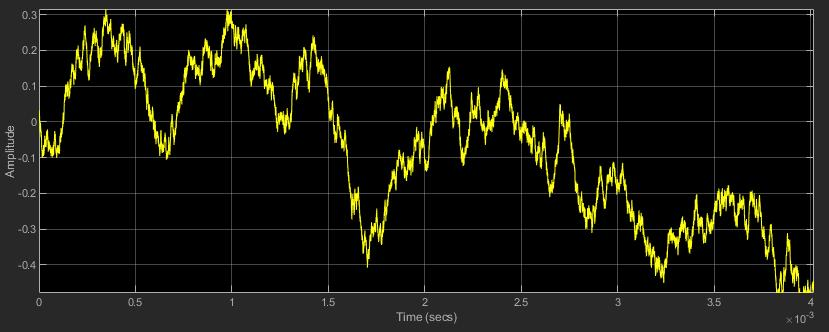
\includegraphics[width = 0.7\textwidth]{images/Ref2Fig2.jpg}
    \end{frame}

	\begin{frame}{\textbf{相位噪声模型}}
		\begin{columns}[T] % align columns
			\begin{column}<0->{.40\textwidth}
				\begin{figure}[thpb]
					\centering
					\resizebox{1\linewidth}{!}{
						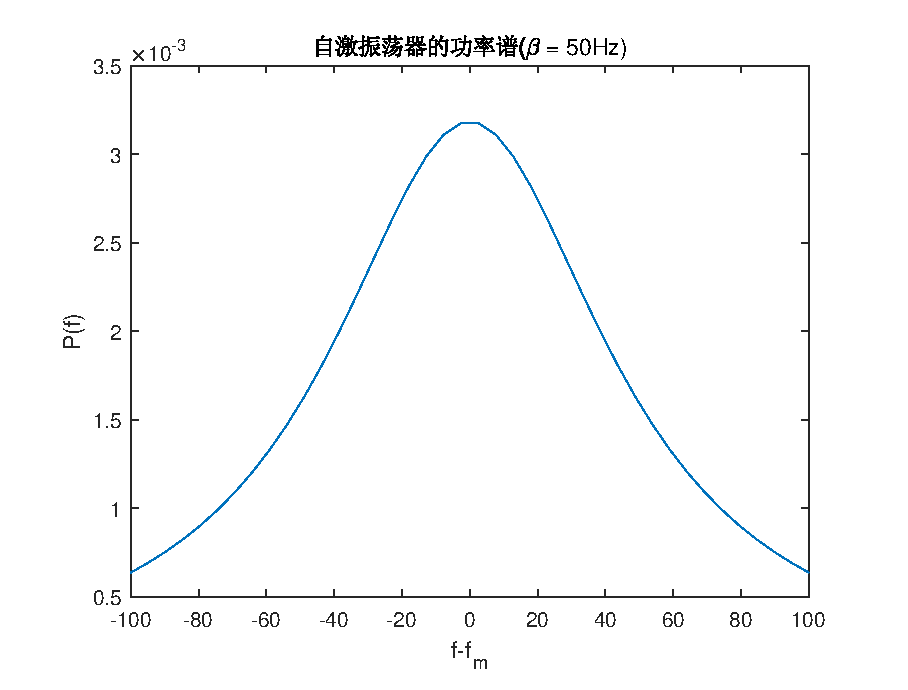
\includegraphics{images/PN.eps}
					}
					%\includegraphics[scale=1.0]{figurefile}
					$\quad$\caption{$\beta=50$Hz时的相位噪声的功率谱}
					\label{fig:campus}
				\end{figure}
			\end{column}%
			\hfill%
			\begin{column}<0->{.5\textwidth}
				\begin{itemize}
					\item 参数$c$表示相位噪声的波动率.
					\item 功率谱密度函数为$P(f) = \frac{c/2}{4{{\pi }^{2}}{{(f-{{f}_{m}})}^{2}}+{{\left( c/2 \right)}^{2}}}$
					\item 复数振荡器输出信号的3-dB带宽为$\beta = \frac{c}{4\pi}$ 
					\item 以$T_s$为时间间隔进行抽样后有$\phi[n+1]-\phi[n]\sim\mathcal{N}(0,cT_s)$
				\end{itemize}
			\end{column}%
		\end{columns}
	\end{frame}

	\begin{frame}{\textbf{小结}}
		\begin{block}{在发送端考虑的RF}
			\begin{itemize}
				\item I/Q不平衡系数:$\alpha_{I,tx}$与$\alpha_{Q,tx}$
				\item 相位的不匹配$\theta_{I,tx}$与$\theta_{Q,tx}$
				\item 相位的噪声过程$\phi_{tx}(t)$
			\end{itemize}
		\end{block}
	
		\begin{block}{在接收端考虑的RF}
		\begin{itemize}
			\item I/Q不平衡系数:$\alpha_{I,rx}$与$\alpha_{Q,rx}$
			\item 相位的不匹配$\theta_{I,rx}$与$\theta_{Q,rx}$
			\item 相位的噪声过程$\phi_{rx}(t)$
		\end{itemize}
		\end{block}
	\end{frame}